\documentclass[11pt,letterpaper]{article}
\usepackage{../assets/scientific_report}
\usepackage{float}
\usepackage{listings}
\usepackage{xcolor}
\usepackage{graphicx}
\usepackage{geometry}
\geometry{headheight=23pt, top=2cm, bottom=2cm, left=2.5cm, right=2.5cm}
\setlength{\parskip}{0.5em}
\setlength{\parindent}{0pt}
\lstset{language=C,basicstyle=\ttfamily\small,keywordstyle=\color{blue}\bfseries,commentstyle=\color{green!60!black}\itshape,numbers=left,numberstyle=\tiny\color{gray},numbersep=8pt,frame=single,breaklines=true,captionpos=b,tabsize=4,showstringspaces=false}
\begin{document}
\pagestyle{plain}
\begin{center}
{\LARGE\bfseries Aplicações Limitadas por Memória e por CPU}\\[0.4em]
{\normalsize Eugênio Vitor Lopes dos Santos}\\[0.3em]
{\small DCA3703 -- Programação Paralela, Universidade Federal do Rio Grande do Norte}\\[0.3em]
\end{center}

\section{Enunciado}
Implemente dois programas paralelos em C com OpenMP: um limitado por memória, com somas simples em vetores, e outro limitado por CPU, com cálculos matemáticos intensivos. Paralelize com \texttt{\#pragma omp parallel for} e meça o tempo de execução variando o número de threads. Analise quando o desempenho melhora, estabiliza ou piora. Reflita sobre como o multithreading de hardware pode ajudar programas memory-bound e atrapalhar programas compute-bound pela competição por recursos.

\section{Fundamentação}
Uma aplicação memory-bound transfere muitos dados e realiza poucas operações por byte. Cada iteração lê dois valores e escreve um valor. O gargalo é a largura de banda da memória. A soma faz uma operação de ponto flutuante para cada 24 bytes transferidos, sem contar efeitos de cache.

Uma aplicação compute-bound realiza muitas operações antes de acessar novos dados. Aqui, cada elemento roda 50 repetições de \texttt{sqrt} e \texttt{sin}. O cálculo dessas funções leva mais tempo que ler e escrever um único elemento. Sem conhecer a implementação da biblioteca matemática, não dá para atribuir um número exato de FLOPs. A classificação depende do comportamento do laço, não de uma estimativa precisa de FLOPs.

Processadores modernos usam arquiteturas heterogêneas com dois tipos de núcleos. Os núcleos P (Performance) têm maior clock, mais unidades de execução e cache maior. Os núcleos E (Efficiency) são menores, com menos unidades de execução e clock inferior, mas consomem menos energia. Um processador como o i7-14700HX combina 8 núcleos P e 6 núcleos E, totalizando 14 núcleos físicos e 28 threads lógicos (Hyper-Threading nos P).

O multithreading de hardware ajuda uma aplicação memory-bound porque, enquanto uma thread espera dados da memória, outra pode executar. O ganho depende da latência e da largura de banda disponíveis. Quando a largura de banda satura, threads adicionais competem pelo mesmo recurso. Em uma aplicação compute-bound, cada thread precisa de unidades de execução. Se há mais threads do que unidades disponíveis, o escalonador do OS distribui o tempo de CPU entre elas, e o speedup fica abaixo do ideal.

\section{Implementação}
O enunciado pede ``dois programas'', mas esta implementação usa um único arquivo e um único executável com dois testes independentes, medidos separadamente. Isso evita repetir código de alocação, inicialização, medição e configuração de threads. Os dois casos exigidos ficam preservados: o primeiro laço é memory-bound e o segundo é compute-bound.

O teste memory-bound aloca os vetores \texttt{A}, \texttt{B} e \texttt{C} e calcula \texttt{C[i] = A[i] + B[i]}. Cada thread escreve em uma posição diferente de \texttt{C}. O teste compute-bound aplica 50 repetições de \texttt{sqrt} e \texttt{sin} a cada elemento de \texttt{V}. A variável temporária \texttt{val} é privada de cada iteração. Alocação e preenchimento dos vetores acontecem antes dos cronômetros. Cada medição cobre somente o seu laço paralelo.
\lstinputlisting[caption={Testes limitado pela memória e limitado pela CPU}]{tarefa04.c}

O arquivo é compilado com GCC, \texttt{-fopenmp} e \texttt{-lm}. O programa recebe o número de elementos como argumento, com $N=50.000.000$ como padrão. Os testes deste relatório usam $N=5.000.000$. A medição usa \texttt{CLOCK\_MONOTONIC}, que não sofre alterações no relógio do sistema. Cada ponto nos gráficos é a \textbf{média de 10 execuções}, com barras de erro indicando o desvio padrão.

\begin{lstlisting}[caption={Compilação e execução dos testes}]
gcc -std=c11 -Wall -Wextra -fopenmp tarefa04.c -o tarefa04 -lm

OMP_NUM_THREADS=1 ./tarefa04 5000000
OMP_NUM_THREADS=28 ./tarefa04 5000000
\end{lstlisting}

\newpage
\section{Resultados e Discussão}

O hardware é um Intel Core i7-14700HX com 14 núcleos físicos (8P+6E) e 28 threads lógicos. Cada ponto nos gráficos é a média de 10 execuções. As barras de erro mostram o desvio padrão.

\begin{figure}[H]
\centering
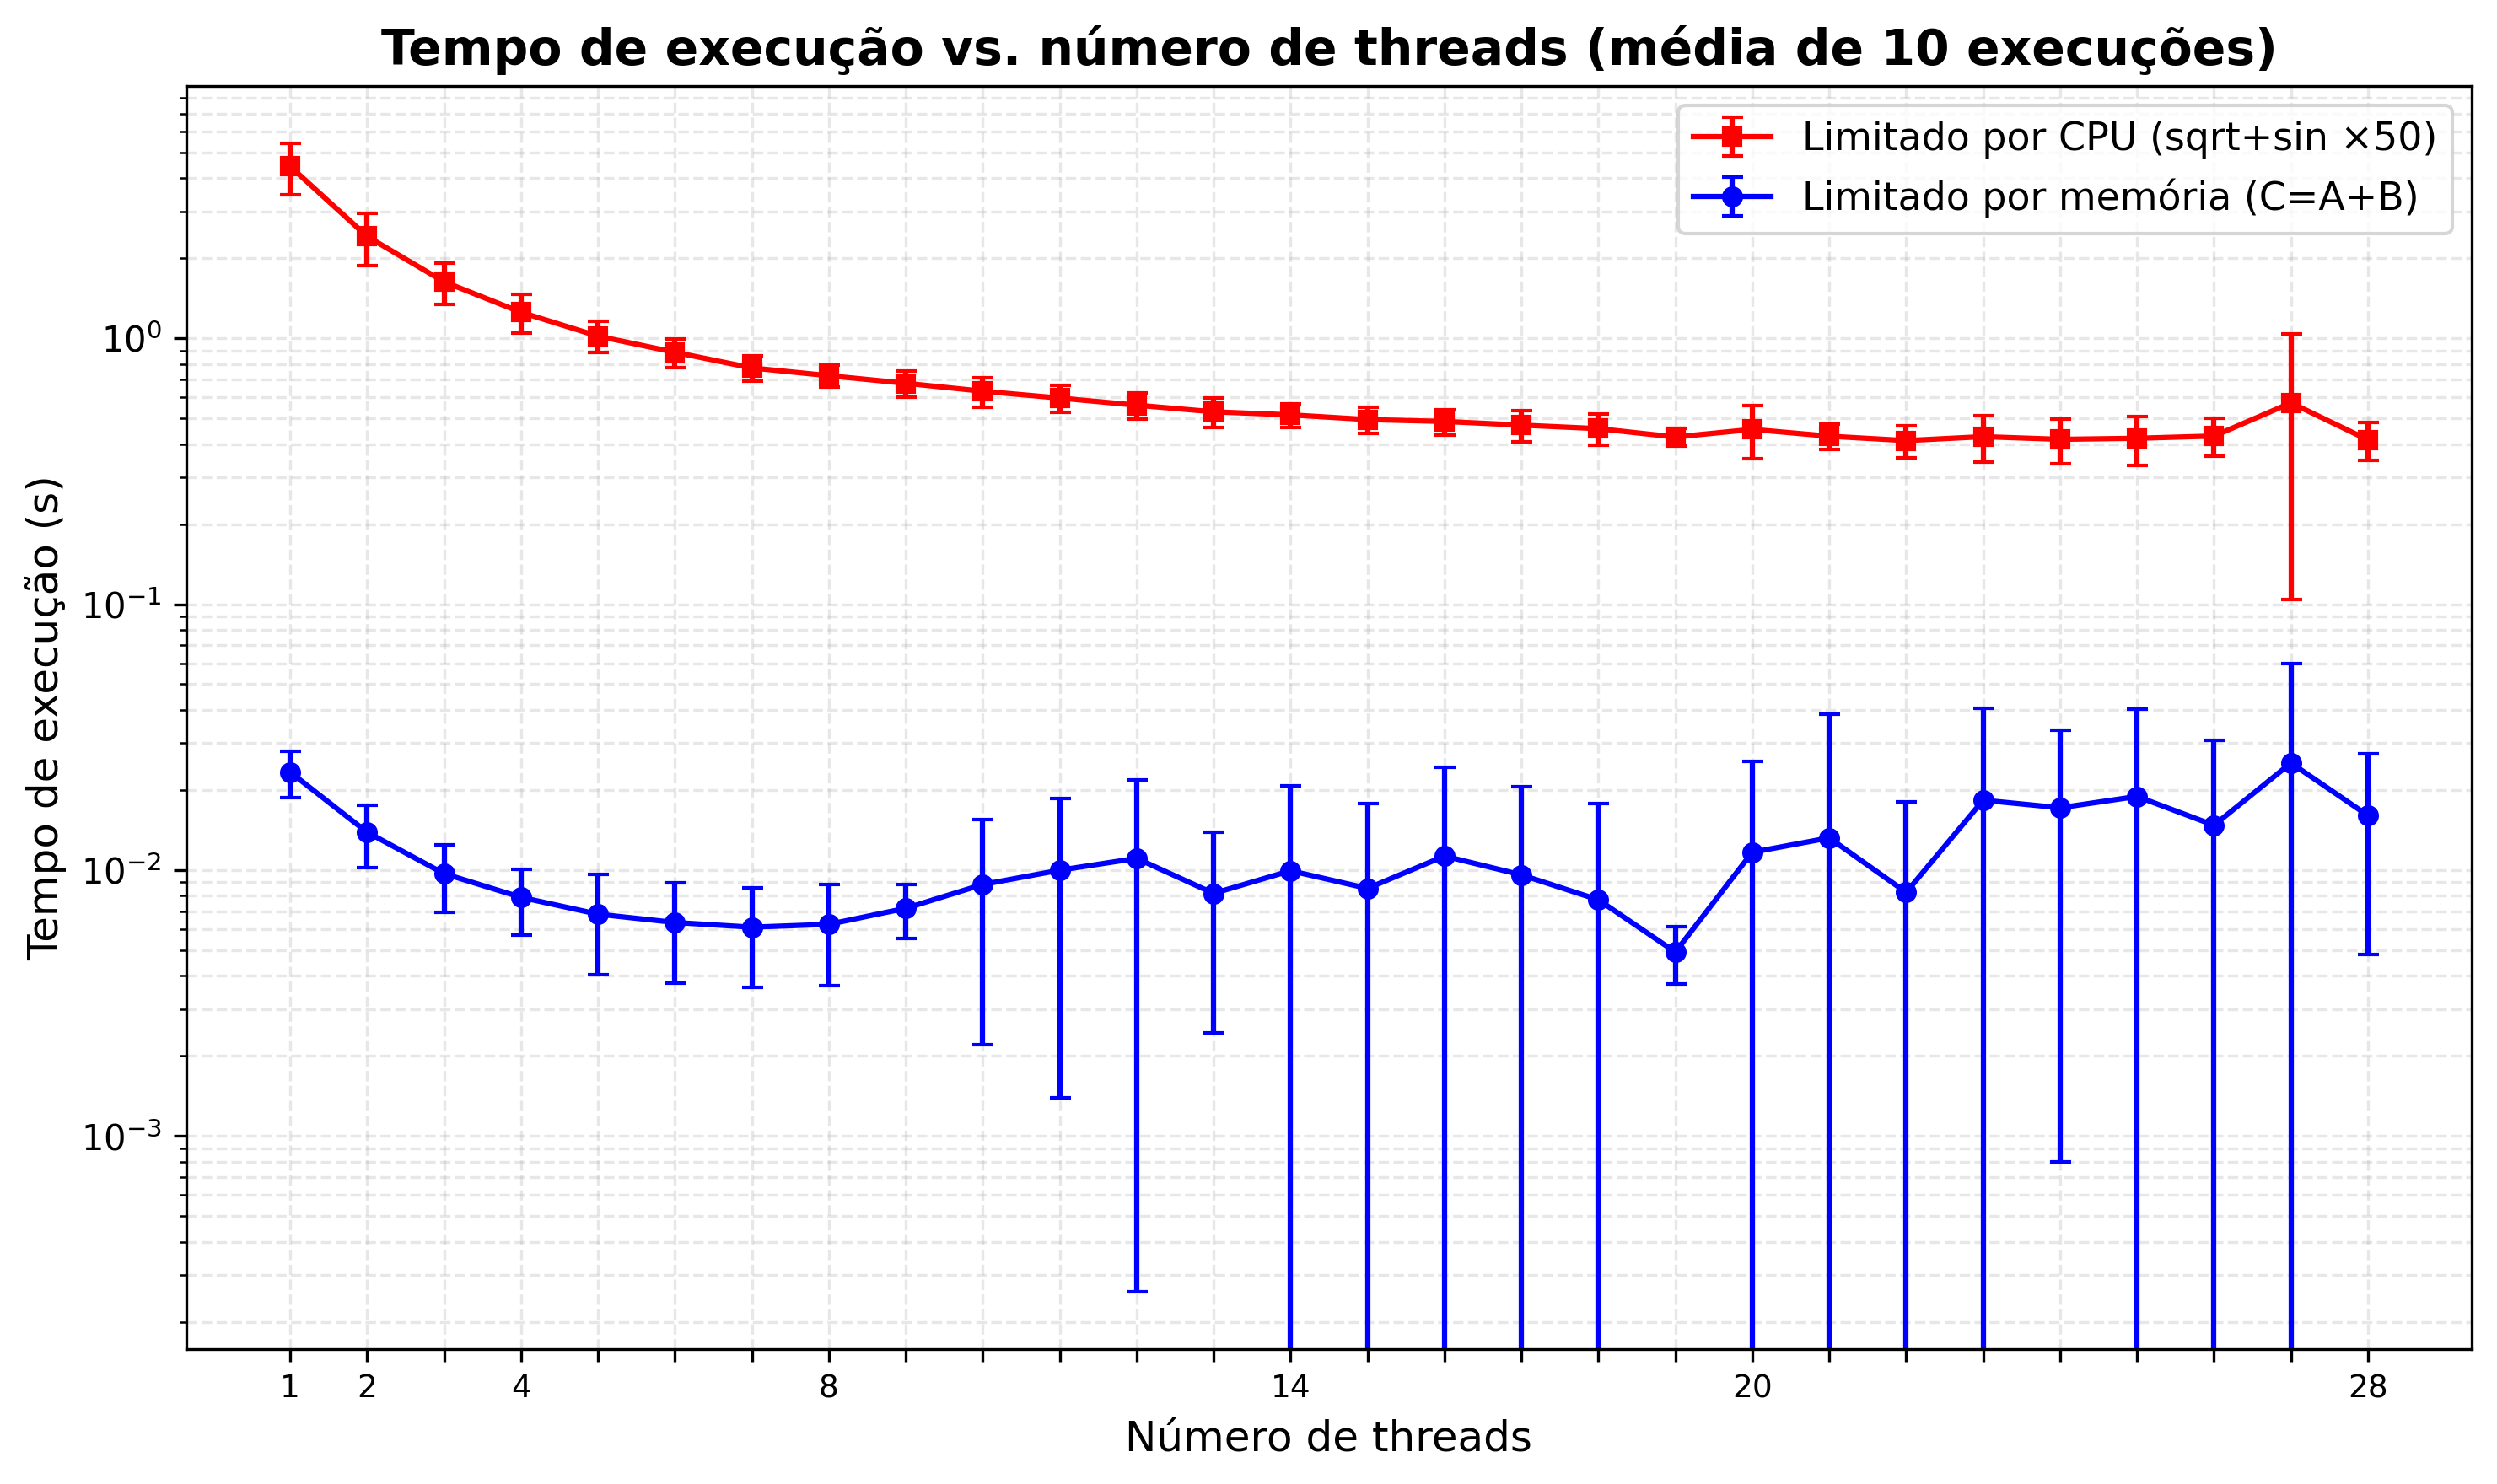
\includegraphics[width=0.9\textwidth]{speedup_plot.png}
\caption{Tempo de execução em função do número de threads (média de 10 execuções com desvio padrão).}
\label{fig:tempos}
\end{figure}

\subsection{Caso memory-bound}

O kernel \texttt{memory\_bound} faz \texttt{C[i] = A[i] + B[i]}, uma adição por elemento. Intensidade aritmética: $1/24 \approx 0{,}042$ FLOP/byte.

Três regiões aparecem nos dados. De T1 a T7, o tempo cai de 23,4\,ms para 6,1\,ms (speedup de 3,83$\times$). Threads adicionais escondem a latência de memória: enquanto uma thread espera dados do controlador, outra executa a soma. De T8 a T18, o tempo estagna entre 6\,ms e 11\,ms, com desvios padrão que crescem de 2\,ms até 13\,ms. De T19 a T28, o tempo médio sobe para 14,9\,ms. O desvio padrão ultrapassa a média em vários pontos. Em T27, o speedup cai para 0,92$\times$: 28 threads são \emph{mais lentas} que uma thread única.

O i7-14700HX tem dois canais DDR5. Quando threads de núcleos P e E competem pelo mesmo barramento, o throughput cai. Além disso, os 6 núcleos E têm cache L2 menor e menor largura de banda de memória que os P. Quando o escalonador do OS aloca threads em núcleos E, a latência de acesso à memória aumenta. Isso explica por que a degradação começa antes de atingir o número total de threads: a partir de T8, thread extras começam a cair nos núcleos E, que são mais lentos tanto em compute quanto em memory access.

Os desvios padrão altos (34\,ms em T27, contra média de 25\,ms) acontecem porque o escalonamento do OS muda a cada execução: às vezes coloca threads favoravelmente nos núcleos P, às vezes nos E, e às vezes mistura. Não há controle sobre qual núcleo roda cada thread.

\subsection{Caso cpu-bound}

O kernel \texttt{cpu\_bound} aplica 50 repetições de \texttt{sqrt} e \texttt{sin} por elemento. Intensidade: $\sim$65,6 FLOP/byte.

O speedup vai de 1,83$\times$ com 2 threads a 10,74$\times$ com 22 threads. De T1 a T8, o ganho é quase linear porque todas as threads rodam nos 8 núcleos P, que têm IPC alto. A partir de T9 (7,45$\times$), o ganho marginal cai porque threads extras passam a ser escalonadas nos 6 núcleos E, que têm menos unidades de execução e cache inferior. O pico de 10,74$\times$ com 22 threads reflete o limite prático: 8 núcleos P dão o ganho principal, os 6 E adicionam pouco porque suas unidades de execução são menores e o cache L2 é compartilhado entre menos threads.

O desvio padrão fica entre 5\,ms e 10\,ms até T26, o que confirma que o cálculo é determinístico. A excessão é T27 (desvio de 467\,ms, média de 572\,ms), provavelmente por interferência de outro processo do sistema em uma das 10 execuções.

\begin{figure}[H]
\centering
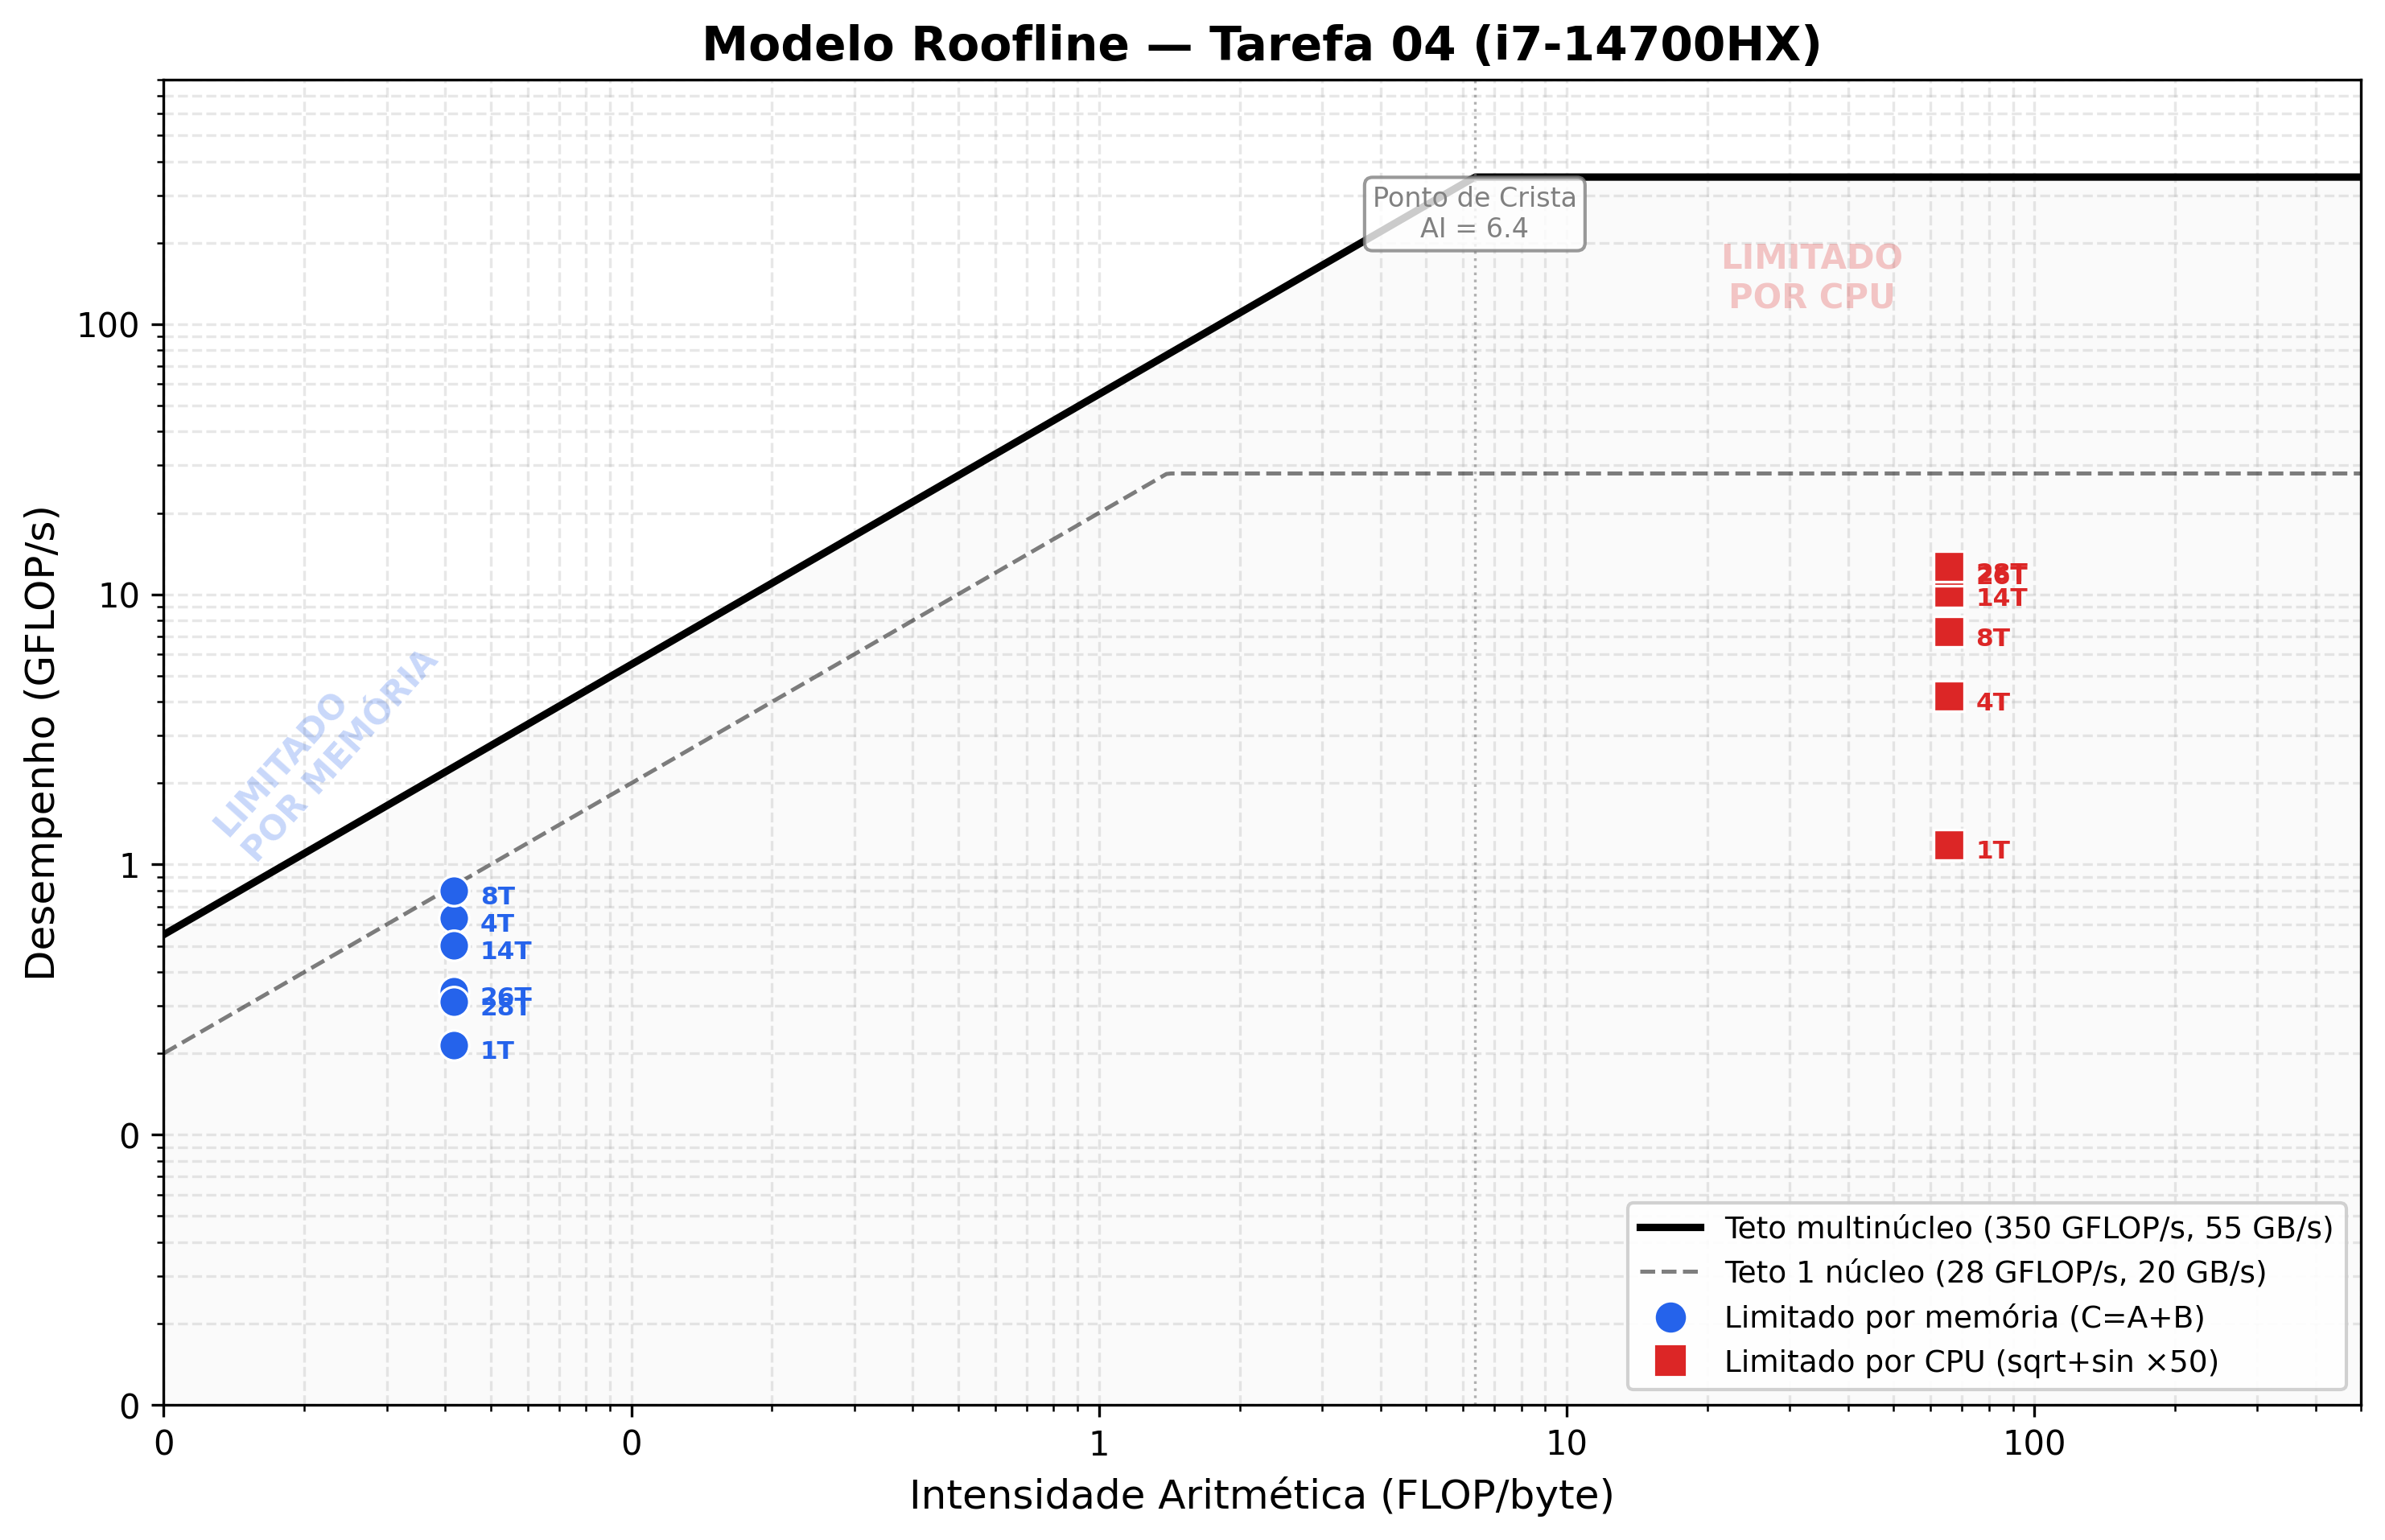
\includegraphics[width=0.9\textwidth]{roofline_plot.png}
\caption{Modelo Roofline ajustado aos resultados com $N=5.000.000$ (média de 10 execuções). Os tetos são estimativas de pico do sistema de referência.}
\label{fig:roofline}
\end{figure}

\newpage
\subsection{Comparação}

O kernel memory-bound faz 1 FLOP a cada 24 bytes. O kernel cpu-bound faz $\sim$1050 FLOPs a cada 16 bytes. O primeiro fica na região memory-bound do Roofline (intensidade bem abaixo do ponto de crista). O segundo fica na região compute-bound (intensidade bem acima).

O resultado: cpu-bound escala quase linearmente com os núcleos. Memory-bound atinge um teto baixo (3,83$\times$) e degrada. Aplicações memory-bound se beneficiam do multithreading até a largura de banda de memória saturar. Depois disso, threads extras competem pelo mesmo barramento e o desempenho cai.

\section{Conclusão}
Os dois testes paralelos usam OpenMP e permitem comparar dois tipos de gargalo. Em uma aplicação memory-bound, o multithreading de hardware ajuda porque, enquanto uma thread aguarda dados da memória, outra pode executar. O ganho existe enquanto a largura de banda da memória não está saturada. Quando múltiplos núcleos lógicos compartilham o mesmo barramento de memória, threads adicionais competem pelo mesmo recurso e os ganhos se estabilizam ou diminuem. Em processadores heterogênicos com núcleos P e E, a degradação é ainda pior porque os núcleos E têm menos largura de banda de memória.

Em uma aplicação compute-bound, o ganho escala bem até atingir os núcleos P. Núcleos E adicionam ganho marginal porque têm menos unidades de execução e cache inferior. O speedup máximo fica longe do ideal teórico de 28$\times$ porque os 6 núcleos E contribuem muito menos que os 8 P.

\end{document}
